\begin{frame}
    \frametitle{Introduzione}
    \addtocounter{nframe}{1}
    
    %\begin{center}
    %    
\includegraphics[width=.2\textwidth]{../imgs/tei-r.pdf}
    %\end{center}

    \begin{block}{Cos'è la TEI}
        la TEI - \textit{acronimo di Text Encoding Initiative} - rappresenta un punto di riferimento per tutte le iniziative il cui scopo principale è quello di digitalizzare risorse testuali in ambito umanistico per fini di ricerca e di conservazione.
    \end{block}
    
\end{frame}

\begin{frame}
  \frametitle{Introduzione}
  \addtocounter{nframe}{1}
  
  %\begin{center}
  %    
\includegraphics[width=.2\textwidth]{../imgs/tei-r.pdf}
  %\end{center}

  \begin{block}{Elementi editoriali}
      \emph{in parte già disponibili nei moduli TEI di base}
      
      \textit{Per la critica testuale indispensabili i moduli}
      \begin{itemize}
          \item \emph{msdescription} descrizione del manoscritto 
          \item \emph{trans} trascrizione di fonti primarie 
          \item \emph{textcrit} apparato critico
          \item \emph{gaiji} caratteri non standard
      \end{itemize}
  \end{block}
  
\end{frame}

%%
\begin{frame}
  \frametitle{Facsimile ed edizione digitale}
  \addtocounter{nframe}{1}
  
  %\begin{center}
  %    
\includegraphics[width=.2\textwidth]{../imgs/tei-r.pdf}
  %\end{center}

  \begin{block}{Tipi di edizione digitale}
      
      \begin{itemize}
          \item \textbf{edizione ipertestuale} 
          \item \textbf{facsimile digitale} 
          \item \textbf{image-based} 
      \end{itemize}
  \end{block}
  
\end{frame}

\begin{frame}
  \frametitle{Facsimile ed edizione digitale}
  \addtocounter{nframe}{1}
  
  %\begin{center}
  %    
\includegraphics[width=.2\textwidth]{../imgs/tei-r.pdf}
  %\end{center}

  \begin{block}{Edizione ipertestuale}
    Prime a essere prodotte, ancora oggi spesso in formato HTML (derivate anche da elaborazioni di documenti TEI XML). 
    \\Formato ideale per edizioni critiche.
    \\Distribuzione sul Web (es.: Biblioteca Digitale Italiana). 
  \end{block}
  
\end{frame}

\begin{frame}
  \frametitle{Facsimile ed edizione digitale}
  \addtocounter{nframe}{1}
  
  %\begin{center}
  %    
\includegraphics[width=.2\textwidth]{../imgs/tei-r.pdf}
  %\end{center}

  \begin{block}{Facsimile digitale}
    Riproduzione del manoscritto basata su scansione digitale.
    \\Distribuzione sul Web (es.: Progetto e-codices)    
  \end{block}
  
\end{frame}

\begin{frame}
  \frametitle{Facsimile ed edizione digitale}
  \addtocounter{nframe}{1}
  
  %\begin{center}
  %    
\includegraphics[width=.2\textwidth]{../imgs/tei-r.pdf}
  %\end{center}

  \begin{block}{Image-based digital edition}
    \textit{Edizione basata su immagini.}
    \\Il testo dell’edizione (diplomatica, interpretativa, critica) con le immagini del
manoscritto
  \end{block}
  
\end{frame}


%%
\begin{frame}
  \frametitle{Facsimile ed edizione digitale}
  \addtocounter{nframe}{1}
  
  %\begin{center}
  %    
\includegraphics[width=.2\textwidth]{../imgs/tei-r.pdf}
  %\end{center}

  \begin{block}{Edizione basata sulle immagini}
      
      \begin{itemize}
          \item Trascrizione collegata alle immagini del manoscritto
          \item Funzionalità principali collegate all'edizione digitale
          \begin{itemize}
            \item immagini in formati e/o risoluzioni diverse 
            \item lente d’ingrandimento
            \item evidenziazione dettagli 
            \item restauro digitale
            \item motore di ricerca testuale
            \item introduzione paleografica/filologica
            \item commento al testo
            \item bibliografia 
          \end{itemize}
      \end{itemize}
  \end{block}
  
\end{frame}

\begin{frame}
  \frametitle{Facsimile ed edizione digitale}
  \addtocounter{nframe}{1}
  
  %\begin{center}
  %    
\includegraphics[width=.2\textwidth]{../imgs/tei-r.pdf}
  %\end{center}

  \begin{block}{Esempio edizione digitale image-based}
    \textit{Electronic Beowulf}
  \end{block}
  
\end{frame}


%% 
\begin{frame}
  \frametitle{Facsimile ed edizione digitale}
  \addtocounter{nframe}{1}
  
  %\begin{center}
  %    
\includegraphics[width=.2\textwidth]{../imgs/tei-r.pdf}
  %\end{center}

  \begin{block}{Edizione digitale di un manoscritto}
      
      \begin{itemize}
          \item \textbf{immagini} del manoscritto
          \item \textbf{trascrizione} del/i testo/i
          \item creazione del \textbf{facsimile digitale}
          \item \textbf{collegamento} testo-immagine
          
      \end{itemize}
  \end{block}
  
\end{frame}

\begin{frame}
  \frametitle{Facsimile ed edizione digitale}
  \addtocounter{nframe}{1}
  
  %\begin{center}
  %    
\includegraphics[width=.2\textwidth]{../imgs/tei-r.pdf}
  %\end{center}

  \begin{block}{Livelli di edizione}
      
      \begin{itemize}
          \item \textbf{edizione diplomatica}
          \item \textbf{edizione diplomatico-interpretativa}
          \item \textbf{edizione critica}
      \end{itemize}
  \end{block}

  \textit{ In caso di singolo manoscritto possiamo avere edizione diplomatica e/o interpretativa}
  
\end{frame}



%%
\begin{frame}
  \frametitle{Facsimile ed edizione digitale}
  \addtocounter{nframe}{1}
  
  %\begin{center}
  %    
\includegraphics[width=.2\textwidth]{../imgs/tei-r.pdf}
  %\end{center}

  \begin{block}{livelli di edizione: diplomatica}
    Trascrizione del testo di un testimone rispettando la disposizione e la grafia originale, senza nessun tipo di correzione (errori manifesti) o altri interventi editoriali (espansione abbreviazioni).
  \end{block}
  
\end{frame}

\begin{frame}
  \frametitle{Facsimile ed edizione digitale}
  \addtocounter{nframe}{1}
  
  %\begin{center}
  %    
\includegraphics[width=.2\textwidth]{../imgs/tei-r.pdf}
  %\end{center}

  \begin{block}{livelli di edizione: diplomatico-interpretativa}
    Sempre rispettando il testo originale, vengono corretti gli errori più evidenti, regolarizzate certe particolarità ortografiche (suddivisione delle parole), espanse le abbreviazioni, etc.
  \end{block}
  
\end{frame}

\begin{frame}
  \frametitle{Facsimile ed edizione digitale}
  \addtocounter{nframe}{1}
  
  %\begin{center}
  %    
\includegraphics[width=.2\textwidth]{../imgs/tei-r.pdf}
  %\end{center}

  \begin{block}{Livelli di edizione: critica}
    Sulla base della collazione di tutte le trascrizioni dei testimoni viene stabilito lo stemma codicum e si tenta di ricostruire il testo originale confrontando le varianti dei testimoni più validi
  \end{block}
  
\end{frame}

%%
\begin{frame}
  \frametitle{Facsimile ed edizione digitale}
  \addtocounter{nframe}{1}
  
  %\begin{center}
  %    
\includegraphics[width=.2\textwidth]{../imgs/tei-r.pdf}
  %\end{center}

  \begin{block}{Esempio livelli di edizione}
    \textit{Vercelli Book}
  \end{block}
  
\end{frame}

%%

\begin{frame}
  \frametitle{Facsimile ed edizione digitale}
  \addtocounter{nframe}{1}
  
  %\begin{center}
  %    
\includegraphics[width=.2\textwidth]{../imgs/tei-r.pdf}
  %\end{center}

  \begin{block}{Rapporto testo-immagine}
      
      \begin{itemize}
          \item \textbf{collegamento mirato (hot-spot)}
          \item \textbf{collegamento generalizzato}
      \end{itemize}
  \end{block}

\end{frame}

\begin{frame}
  \frametitle{Facsimile ed edizione digitale}
  \addtocounter{nframe}{1}
  
  %\begin{center}
  %    
\includegraphics[width=.2\textwidth]{../imgs/tei-r.pdf}
  %\end{center}

  \begin{block}{Collegamento mirato (hot-spot)}
    Una specifica area dell’immagine viene evidenziata in maniera tale che, interagendo con la stessa, vengono visualizzate delle informazioni quali note editoriali, versione migliorata di un dettaglio, commento al testo, etc.
  \end{block}
  
\end{frame}

\begin{frame}
  \frametitle{Facsimile ed edizione digitale}
  \addtocounter{nframe}{1}
  
  %\begin{center}
  %    
\includegraphics[width=.2\textwidth]{../imgs/tei-r.pdf}
  %\end{center}

  \begin{block}{Collegamento generalizzato}
    Tutto il testo dell’edizione viene messo in relazione diretta con le immagini, o parti di immagine, corrispondenti, in modo da poter accedere facilmente alla porzione di immagine corrispondente partendo dal testo, e viceversa.
  \end{block}
  
\end{frame}



%%
\begin{frame}
  \frametitle{Facsimile ed edizione digitale}
  \addtocounter{nframe}{1}
  
  %\begin{center}
  %    
\includegraphics[width=.2\textwidth]{../imgs/tei-r.pdf}
  %\end{center}

  \begin{block}{Obiettivo}
    Realizzare un collegamento fra testo e immagine in maniera tale che cliccando sul testo viene visualizzata la parte di immagine corrispondente e viceversa
  \end{block}
  
\end{frame}

\begin{frame}
  \frametitle{Facsimile ed edizione digitale}
  \addtocounter{nframe}{1}
  
  %\begin{center}
  %    
\includegraphics[width=.2\textwidth]{../imgs/tei-r.pdf}
  %\end{center}

  \begin{block}{Edizione digitale Facsimile}
    Gli schemi di codifica TEI versione P5 (2007) introducono numerosi miglioramenti per quanto riguarda la gestione e trascrizione di manoscritti
  \end{block}

  \textit{Tra queste la nuova sezione Digital facsimiles nel capitolo 11 Representation of Primary Sources: \url{http://www.tei-c.org/release/doc/tei-p5-doc/en/html/PH.html}}

  
\end{frame}


%%
%modulo per la descrizione di manoscritti (10 Manuscript
%Description http://www.tei-c.org/release/doc/tei-p5-doc/en/html/MS.html)
%nuovo elemento <choice> da usare per le coppie di elementi
%di tipo “editoriale”

%%

\begin{frame}
  \frametitle{Facsimile ed edizione digitale}
  \addtocounter{nframe}{1}
  
  %\begin{center}
  %    
\includegraphics[width=.2\textwidth]{../imgs/tei-r.pdf}
  %\end{center}

  \begin{block}{Edizione digitale Facsimile}
    Includendo il modulo transcr nello schema di codifica TEI si rende disponibile un attributo globale \texttt{@facs}
  \end{block}
  \begin{block}{Edizione digitale Facsimile}
    \textit{\texttt{@facs (facsimile)} points to all or part of an image which corresponds with the content of the element}
  \end{block}

\end{frame}

\begin{frame}
  \frametitle{Facsimile ed edizione digitale}
  \addtocounter{nframe}{1}
  
  %\begin{center}
  %    
\includegraphics[width=.2\textwidth]{../imgs/tei-r.pdf}
  %\end{center}

  \begin{block}{Edizione digitale Facsimile}
    Questo attributo può essere usato in qualsiasi elemento per associare il contenuto dello stesso a un’immagine
  \end{block}
  \begin{block}{Edizione digitale Facsimile: esempi}
    \texttt{<p n="1" facs="para1.jpg" >}
    \\\texttt{<head facs="head.jpg" >}
    \\\texttt{<pb facs="page1.jpg" />}
  \end{block}

\end{frame}


%%

\begin{frame}
  \frametitle{Facsimile ed edizione digitale}
  \addtocounter{nframe}{1}
  
  %\begin{center}
  %    
\includegraphics[width=.2\textwidth]{../imgs/tei-r.pdf}
  %\end{center}

\textbf{oltre a \texttt{@facs} è necessario usare gli altri elementi del modulo transcrption per collegare testo a immagine}
  \begin{block}{Edizione image-based}
      
      \begin{itemize}
          \item \texttt{<facsimile>}
          \item \texttt{<surface>}
          \item \texttt{<zone>}
      \end{itemize}
  \end{block}

\end{frame}


\begin{frame}
  \frametitle{Facsimile ed edizione digitale}
  \addtocounter{nframe}{1}
  
  %\begin{center}
  %    
\includegraphics[width=.2\textwidth]{../imgs/tei-r.pdf}
  %\end{center}

\textbf{oltre a \texttt{@facs} è necessario usare i altri elementi dl modulo transcrption per collegare testo a immagine}
  \begin{block}{Elemento Facsimile}
      
      \begin{itemize}
          \item \texttt{<facsimile>} 
          \item[] contains a representation of some written source in the form of a set of images rather than as transcribed or encoded text.
      \end{itemize}
  \end{block}

\end{frame}

\begin{frame}
  \frametitle{Facsimile ed edizione digitale}
  \addtocounter{nframe}{1}
  
  %\begin{center}
  %    
\includegraphics[width=.2\textwidth]{../imgs/tei-r.pdf}
  %\end{center}

\textbf{oltre a \texttt{@facs} è necessario usare i altri elementi dl modulo transcrption per collegare testo a immagine}
  \begin{block}{Elemento Facsimile}
      
      \begin{itemize}
          \item \texttt{<surface>}
          \item[] defines a written surface in terms of a rectangular coordinate space, optionally grouping one or more graphic representations of that space, and rectangular zones of interest within it.
      \end{itemize}
  \end{block}

  \textit{L'attributo \texttt{@start} points to an element which encodes the starting position of the text corresponding to the inscribed part of the surface.}


\end{frame}

\begin{frame}
  \frametitle{Facsimile ed edizione digitale}
  \addtocounter{nframe}{1}
  
  %\begin{center}
  %    
\includegraphics[width=.2\textwidth]{../imgs/tei-r.pdf}
  %\end{center}

\textbf{oltre a \texttt{@facs} è necessario usare i altri elementi dl modulo transcrption per collegare testo a immagine}
  \begin{block}{Elemento Facsimile}
      
      \begin{itemize}
          \item \texttt{<surface>}
          \item[] defines a written surface in terms of a rectangular coordinate space, optionally grouping one or more graphic representations of that space, and rectangular zones of interest within it.
      \end{itemize}
  \end{block}

\end{frame}

\begin{frame}
  \frametitle{Facsimile ed edizione digitale}
  \addtocounter{nframe}{1}
  
  %\begin{center}
  %    
\includegraphics[width=.2\textwidth]{../imgs/tei-r.pdf}
  %\end{center}

\textbf{oltre a \texttt{@facs} è necessario usare i altri elementi dl modulo transcrption per collegare testo a immagine}
  \begin{block}{Elemento Facsimile}
      
      \begin{itemize}
          \item \texttt{<zone>}
          \item[] defines a rectangular area contained within a surface element.          .
      \end{itemize}
  \end{block}

\end{frame}


%%
\begin{frame}
  \frametitle{Facsimile ed edizione digitale}
  \addtocounter{nframe}{1}
  
  %\begin{center}
  %    
\includegraphics[width=.2\textwidth]{../imgs/tei-r.pdf}
  %\end{center}

  \begin{block}{Elemento Facsimile}
    L’elemento \texttt{<facsimile>} è di tipo strutturale e si pone allo stesso livello di \texttt{<text>} o addirittura in alternativa a quest’ultimo
  \end{block}

  \begin{block}{Elemento Facsimile}
    La TEI permette una \textbf{grande flessibilità}: facsimile digitale con le immagini del ms, facsimile digitale con trascrizione del testo e facsimile digitale con trascrizione e collegamento all'immagine.
  \end{block}

\end{frame}
 
\begin{frame}
  \frametitle{Facsimile ed edizione digitale}
  \addtocounter{nframe}{1}
  
  %\begin{center}
  %    
\includegraphics[width=.2\textwidth]{../imgs/tei-r.pdf}
  %\end{center}

\textit{}{Quando il modulo transcr viene aggiunto allo schema di codifica è possibile scegliere fra:}

  \begin{block}{Elemento Facsimile}
      
      \begin{itemize}
          \item \texttt{un <teiHeader> e un <facsimile>}
          \item \texttt{un <teiHeader> e un <text>}
          \item \texttt{un <teiHeader>, un <facsimile> e un <text>}         .
      \end{itemize}
  \end{block}

\end{frame}


%%
\begin{frame}
  \frametitle{Facsimile ed edizione digitale}
  \addtocounter{nframe}{1}
  
  %\begin{center}
  %    
\includegraphics[width=.2\textwidth]{../imgs/tei-r.pdf}
  %\end{center}

  \begin{block}{Elemento Facsimile}
    \texttt{<TEI>}
    \\\texttt{<teiHeader>}
    \\\texttt{<!-- ... -->}
    \\\texttt{</teiHeader>}
    \\\texttt{<facsimile>}
     \\\texttt{ <graphic url="page1.png"/>}
     \\\texttt{ <graphic url="page2.png"/>}
     \\\texttt{ <graphic url="page3.png"/>}
     \\\texttt{ <graphic url="page4.png"/>}
    \\\texttt{</facsimile>}
   \\\texttt{</TEI>}
  \end{block}

\end{frame}


%%
\begin{frame}
  \frametitle{Facsimile ed edizione digitale}
  \addtocounter{nframe}{1}
  
  %\begin{center}
  %    
\includegraphics[width=.2\textwidth]{../imgs/tei-r.pdf}
  %\end{center}

  \begin{block}{Elemento Facsimile}
    \texttt{<TEI>}
    \\\texttt{<teiHeader>}
    \\\texttt{<!-- ... -->}
    \\\texttt{</teiHeader>}
    \\\texttt{<text>}
     \\\texttt{ <pb facs="page1.png"/>}
     \\\texttt{ <!-- inserire qui il testo di pagina 1 -->}
     \\\texttt{ <pb facs="page2.png"/>}
     \\\texttt{ <!-- inserire qui il testo di pagina 2 -->}
    \\\texttt{</text>}
   \\\texttt{</TEI>}
  \end{block}

\end{frame}

%%
\begin{frame}
  \frametitle{Facsimile ed edizione digitale}
  \addtocounter{nframe}{1}
  
  %\begin{center}
  %    
\includegraphics[width=.2\textwidth]{../imgs/tei-r.pdf}
  %\end{center}

  \begin{block}{Elemento Facsimile}
    Grazie a un foglio di stile XSLT è possibile generare una pagina HMTL divisa in due riquadri (immagine e testo)
  \end{block}
  \begin{block}{Elemento Facsimile}
    Nessun collegamento testo-immagine a livello diverso dalla pagina e non è possibile nemmeno individuare aree particolari delle immagini.  
    \\In fine, i puntatori alle immagini sono sparsi per tutto il documento.
  \end{block}

\end{frame}

%%
\begin{frame}
  \frametitle{Facsimile ed edizione digitale}
  \addtocounter{nframe}{1}
  
  %\begin{center}
  %    
\includegraphics[width=.2\textwidth]{../imgs/tei-r.pdf}
  %\end{center}

  \begin{block}{Elemento Facsimile}
    La soluzione più efficace è la parallel transcription basata su \texttt{<facsimile> e <text>} e all'uso di \texttt{<surface> e <zone>} all’interno di \texttt{<facsimile>.}
  \end{block}
  \begin{block}{Elemento Facsimile}
    Possibilità di definire le aree delle immagini e collegare il testo della trascrizione a tali aree e/o immagini secondarie.
  \end{block}

\end{frame}



%%
\begin{frame}
  \frametitle{Facsimile ed edizione digitale}
  \addtocounter{nframe}{1}
  
  %\begin{center}
  %    
\includegraphics[width=.2\textwidth]{../imgs/tei-r.pdf}
  %\end{center}

  \begin{block}{Elemento Facsimile}
    Le aree delle immagini sono individuate per mezzo di un sistema di coordinate cartesiane registrate come valori di attributi di \texttt{<surface> e <zone>}.
  \end{block}
  \begin{block}{Coordinate area immagini}
    \begin{itemize}
      \item \textbf{ulx, uly} coordinate x e y dell’angolo superiore sinistro 
      \item \textbf{lrx, lry} coordinate x e y dell’angolo inferiore destro
    \end{itemize}

  \end{block}

\end{frame}



%%
\begin{frame}
  \frametitle{Facsimile ed edizione digitale}
  \addtocounter{nframe}{1}
  
  %\begin{center}
  %    
\includegraphics[width=.2\textwidth]{../imgs/tei-r.pdf}
  %\end{center}

  \begin{block}{Elemento Surface}
    \texttt{<surface>} individua la superficie scritta di un’immagine
  \end{block}
  \begin{block}{Elemento Surface: esempio}
    
    \texttt{<surface ulx="0" uly="0" lrx="400" lry="280" >} 
    \\\texttt{ <graphic url="page1.png"/>}
    \\\texttt{</surface>}

  \end{block}

\end{frame}

\begin{frame}
  \frametitle{Facsimile ed edizione digitale}
  \addtocounter{nframe}{1}
  
  %\begin{center}
  %    
\includegraphics[width=.2\textwidth]{../imgs/tei-r.pdf}
  %\end{center}

  \begin{block}{Elemento Surface}
    può contenere più di un elemento \texttt{<graphic>}
  \end{block}
  \begin{block}{Elemento Surface: esempio}
    
    \texttt{<surface>}
    \texttt{ <graphic url="page1-highRes.png"/> }
    \texttt{ <graphic url="page1-lowRes.png"/>}
    \texttt{</surface>}

  \end{block}
  \textit{\texttt{<surface>} stesso si trova all’interno di \texttt{<facsimile>}}
\end{frame}



%%

\begin{frame}
  \frametitle{Facsimile ed edizione digitale}
  \addtocounter{nframe}{1}
  
  %\begin{center}
  %    
\includegraphics[width=.2\textwidth]{../imgs/tei-r.pdf}
  %\end{center}
\textit{l'elemento facsimile invece di \texttt{<graphic>} può contenere una o più \texttt{<zone>}}

  \begin{block}{Elemento Zone}
    
    \texttt{<zone>} definisce una specifica area dell’immagine usando lo stesso sistema di coordinate di \texttt{<surface>}

  \end{block}
  \begin{block}{Elemento Zone: esempio}
    \texttt{<surface ulx="0" uly="0" lrx="500" lry="321" >}
    \\\texttt{ <zone ulx="50" uly="20" lrx="400" lry="280" >}
    \\\texttt{ <graphic url="scrittura.png"/>}
    \\\texttt{ </zone>}
    \\\texttt{ <note>first page</note>}
    \\\texttt{</surface>}
  \end{block}
  \texttt{<surface>} stesso si trova all’interno di \texttt{<facsimile>}
\end{frame}

%o una porzione più piccola (utile per creare un hot-spot):

%<zone ulx="120" uly="48" lrx="143" lry="56">
% <graphic url="gloss.png"/>
% <note>Scribe gloss</note>
%</zone>

%%
\begin{frame}
  \frametitle{Facsimile ed edizione digitale}
  \addtocounter{nframe}{1}
  
  \begin{center}
    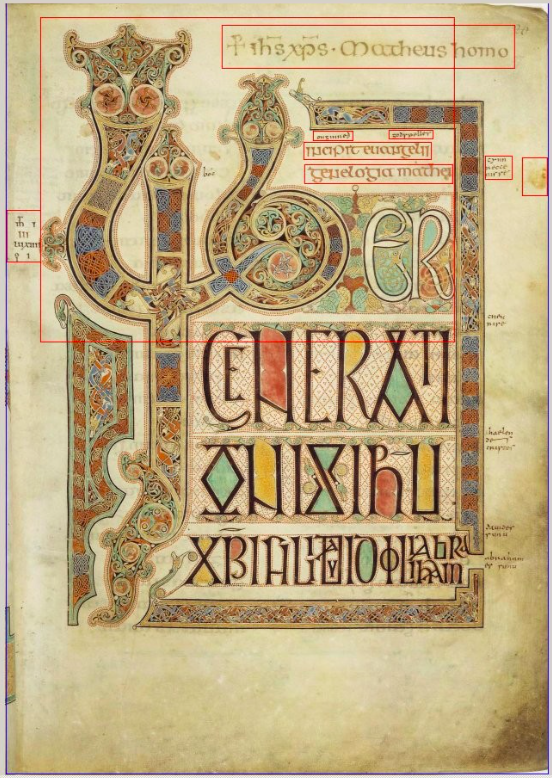
\includegraphics[width=.9\textwidth]{imgs/AreeZoneManoscritto.png}
  \end{center}
\end{frame}

%%
\begin{frame}
  \frametitle{Facsimile ed edizione digitale}
  \addtocounter{nframe}{1}
  
  \begin{block}{Esempio facsimile zone}
    \texttt{<facsimile xml:id="imtAnnotatedImage" > <surface>
    <graphic height="1797px" url="LindisfarneFol27rIncipitMatt.jpg" width="1266px"/>
    <zone lrx="1268" lry="1797" rend="visible" rendition="surface" ulx="0" uly="4" xml:id="imtArea-0"/>
    <zone lrx="1267" lry="450" rend="visible" rendition="zone" ulx="1202" uly="356" xml:id="imtArea-1"/>
    <zone lrx="1050" lry="792" rend="visible" rendition="zone" ulx="81" uly="30" xml:id="imtArea-3"/>
    <zone lrx="1190" lry="154" rend="visible" rendition="zone" ulx="503" uly="48" xml:id="imtArea-4"/>
    <!-- altre zone -->
    </surface></facsimile>}
  \end{block}

\end{frame}


%%
\begin{frame}
  \frametitle{Facsimile ed edizione digitale}
  \addtocounter{nframe}{1}
  
  %\begin{center}
  %    
\includegraphics[width=.2\textwidth]{../imgs/tei-r.pdf}
  %\end{center}

  \begin{block}{Collegare il testo alle immagini}
    Per collegare il testo della trascrizione alle aree corrispondenti dell’immagine bisogna \textbf{assegnare un identificatore univoco} a \textit{ciascun elemento del facsimile} usando \textbf{l’attributo xml:id}.  
\end{block}

  \begin{block}{Collegare il testo alle immagini}
    
    Usare l’attributo \textbf{facs} negli elementi testuali per \textbf{specificare l’id} degli elementi \texttt{<surface> e <zone>} corrispondenti

  \end{block}
\end{frame}

\begin{frame}
  \frametitle{Facsimile ed edizione digitale}
  \addtocounter{nframe}{1}
  
  %\begin{center}
  %    
\includegraphics[width=.2\textwidth]{../imgs/tei-r.pdf}
  %\end{center}

  \begin{block}{Collegare le immagini al testo}
    Per collegare le aree delle immagini ai corrispondenti elementi di testo bisogna
    assegnare un \textbf{identificatore univoco} a \textit{ciascun elemento della trascrizione} usando l’\textbf{attributo xml:id}
  \end{block}

  \begin{block}{Collegare le immagini al testo}
    Usare l’attributo \textbf{start} negli elementi \texttt{<surface> e <zone>} per \textbf{specificare l’id} degli \textit{elementi testuali corrispondenti}.
  \end{block}
\end{frame}



%%

\begin{frame}
  \frametitle{Facsimile ed edizione digitale}
  \addtocounter{nframe}{1}
  
  \begin{block}{Esempio collegamento completo}
    \texttt{<text>
    <body>
     <div>
   <pb facs="\#page1" n="1" xml:id="page-1"/>
   <p>Lorem ipsum ... <gloss facs="\#det1" >semper</gloss></p> </div>
    </body>
   </text>
   <facsimile>
   <surface xml:id="page1” start="\#page-1" ulx="0" uly="0" lrx="500" lry="321" >
   <graphic url="page1.png”>
   <zone xml:id="line1" ulx="50" uly="80" lrx="200" lry="321" >
   <graphic url="line1.png"/>
   <note>First page.</note> </zone>
   <zone xml:id="det1" ulx="120" uly="48" lrx="143" lry="56" > <graphic url="gloss.png"/>
   <note>Scribe gloss.</note>
     </zone>
    </surface>
   </facsimile>}
  \end{block}

\end{frame}


%%
\begin{frame}
  \frametitle{Facsimile ed edizione digitale}
  \addtocounter{nframe}{1}
  
  %\begin{center}
  %    
\includegraphics[width=.2\textwidth]{../imgs/tei-r.pdf}
  %\end{center}

  \begin{block}{Eembedded transcription}
    Un metodo a metà fra facsimile digitale e edizione basata su immagini è quello della embedded transcription.
    \\\texttt{http://www.tei-c.org/release/doc/tei-p5-doc/en/html/PH.html\#PHZLAB}
  \end{block}

  \begin{block}{Differenza con il metodo parallel transcription}
    Il testo è considerato di accompagnamento, il focus infatti e sulle immagini (ad esempio disposizione fisica delle parti).
  \end{block}
\end{frame}




%%

\begin{frame}
  \frametitle{Facsimile ed edizione digitale}
  \addtocounter{nframe}{1}
  
  %\begin{center}
  %    
\includegraphics[width=.2\textwidth]{../imgs/tei-r.pdf}
  %\end{center}

  \begin{block}{Embedded transcription}
    Un metodo a metà fra facsimile digitale e edizione basata su immagini è quello della embedded transcription.
    \\\texttt{http://www.tei-c.org/release/doc/tei-p5-doc/en/html/PH.html\#PHZLAB}
  \end{block}

  \begin{block}{Differenza con il metodo parallel transcription}
    Il testo è considerato di accompagnamento, il focus infatti e sulle immagini (ad esempio disposizione fisica delle parti).
  \end{block}
\end{frame}

%%

\begin{frame}
  \frametitle{Facsimile ed edizione digitale}
  \addtocounter{nframe}{1}
  
  %\begin{center}
  %    
\includegraphics[width=.2\textwidth]{../imgs/tei-r.pdf}
  %\end{center}

  \begin{block}{Embedded transcription}
    Per implementare il metodo si usa l’elemento \texttt{<sourceDoc>} sullo stesso livello gerarchico e in alternativa a \texttt{<facsimile> e <text>}.
  \end{block}

  \begin{block}{Embedded transcription}
    All'interno di \texttt{<sourceDoc>} gli elementi \texttt{<surface> e <zone>} vengono utilizzati in maniera simile a quanto visto per l'elemento \texttt{<facsimile>}.
  \end{block}
\end{frame}

\begin{frame}
  \frametitle{Facsimile ed edizione digitale}
  \addtocounter{nframe}{1}
  
  %\begin{center}
  %    
\includegraphics[width=.2\textwidth]{../imgs/tei-r.pdf}
  %\end{center}

  \begin{block}{Embedded transcription}
    L'elemento \texttt{<zone>} contiene una serie di elementi \texttt{<line>} corrispondenti alle righe di testo
  \end{block}

  \begin{block}{Embedded transcription: esempio}
    \texttt{<zone ulx="20" uly="40" lrx="120" lry="180" >}
   \\\texttt{ <line>prima riga di trascrizione</line>}
   \\\texttt{ <line>seconda riga di trascrizione</line>}
   \\\texttt{</zone>}
  \end{block}
\textit{Il content model di \texttt{<line>} è limitato e con ci sono conflitti di gerarchie
}\end{frame}



%%

\begin{frame}
  \frametitle{Facsimile ed edizione digitale}
  \addtocounter{nframe}{1}
  
  %\begin{center}
  %    
\includegraphics[width=.2\textwidth]{../imgs/tei-r.pdf}
  %\end{center}

  \begin{block}{Eembedded transcription}
    \begin{center}
        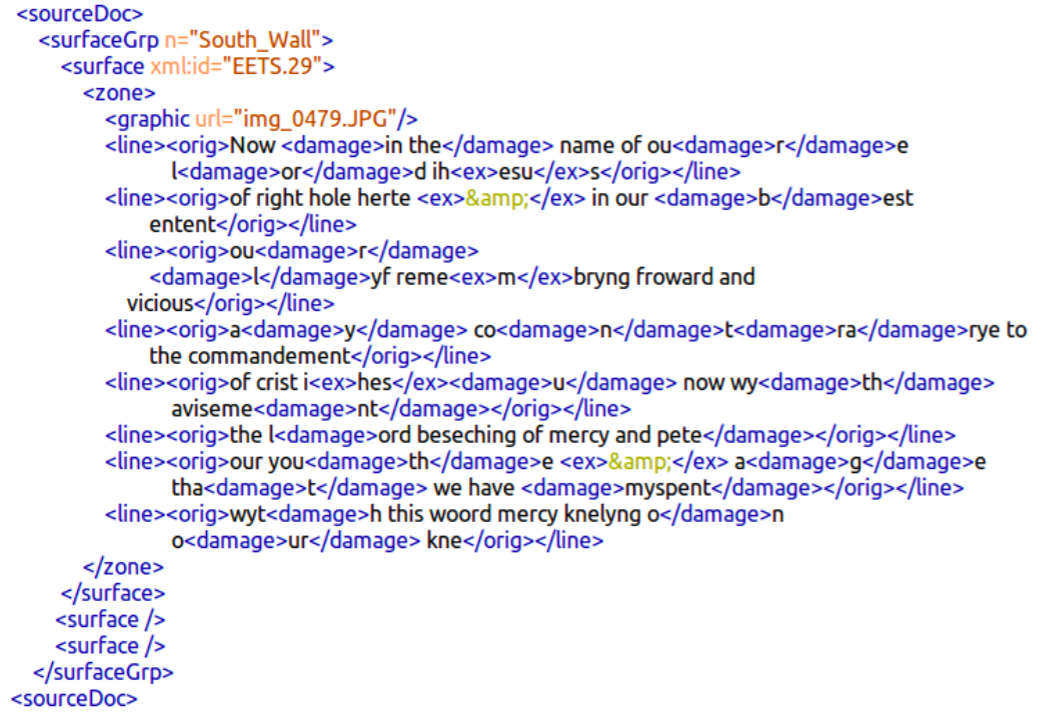
\includegraphics[width=.9\textwidth]{imgs/EsempioEmbeddedTranscription.png}
    \end{center}
  \end{block}

  \begin{block}{Differenza con il metodo parallel transcription}
    \textbf{Esempio Taccuini di Proust}
  \end{block}
\end{frame}



%%

\begin{frame}
  \frametitle{Facsimile ed edizione digitale}
  \addtocounter{nframe}{1}
  
  %\begin{center}
  %    
\includegraphics[width=.2\textwidth]{../imgs/tei-r.pdf}
  %\end{center}

  
    \textit{Esistono numerosi programmi per calcolare le coordinate di aree su immagini facsimile.}
  
  \begin{block}{Come inserire le coordinate}
    Software di disegno in formato bitmap strumenti per programmatori di siti web.
    \\Software progettati per creatori di edizioni digitali (\textit{EPPT}).
  \end{block}

\end{frame}

%%

\begin{frame}
  \frametitle{Facsimile ed edizione digitale}
  \addtocounter{nframe}{1}
  
  %\begin{center}
  %    
\includegraphics[width=.2\textwidth]{../imgs/tei-r.pdf}
  %\end{center}

  \begin{block}{Strumenti per per immagini facsimile}
   Un utile strumento per ottenere le coordinate di regioni di interesse in formato TEI è \textbf{TEIzoner}.
  \end{block}
\end{frame}


%%

\begin{frame}
  \frametitle{Facsimile ed edizione digitale}
  \addtocounter{nframe}{1}
  
  %\begin{center}
  %    
\includegraphics[width=.2\textwidth]{../imgs/tei-r.pdf}
  %\end{center}

  \begin{block}{Edizioni image-based: Esercizio}
   \textbf{ Codificare lettera Bellini}
  \end{block}

\end{frame}


